\begin{columns}[t]
	\begin{column}{0.70\textwidth}
		\begin{block}{\large Pose Estimation using Monte Carlo Tree Search}
			\centering
			\begin{figure}[h]
				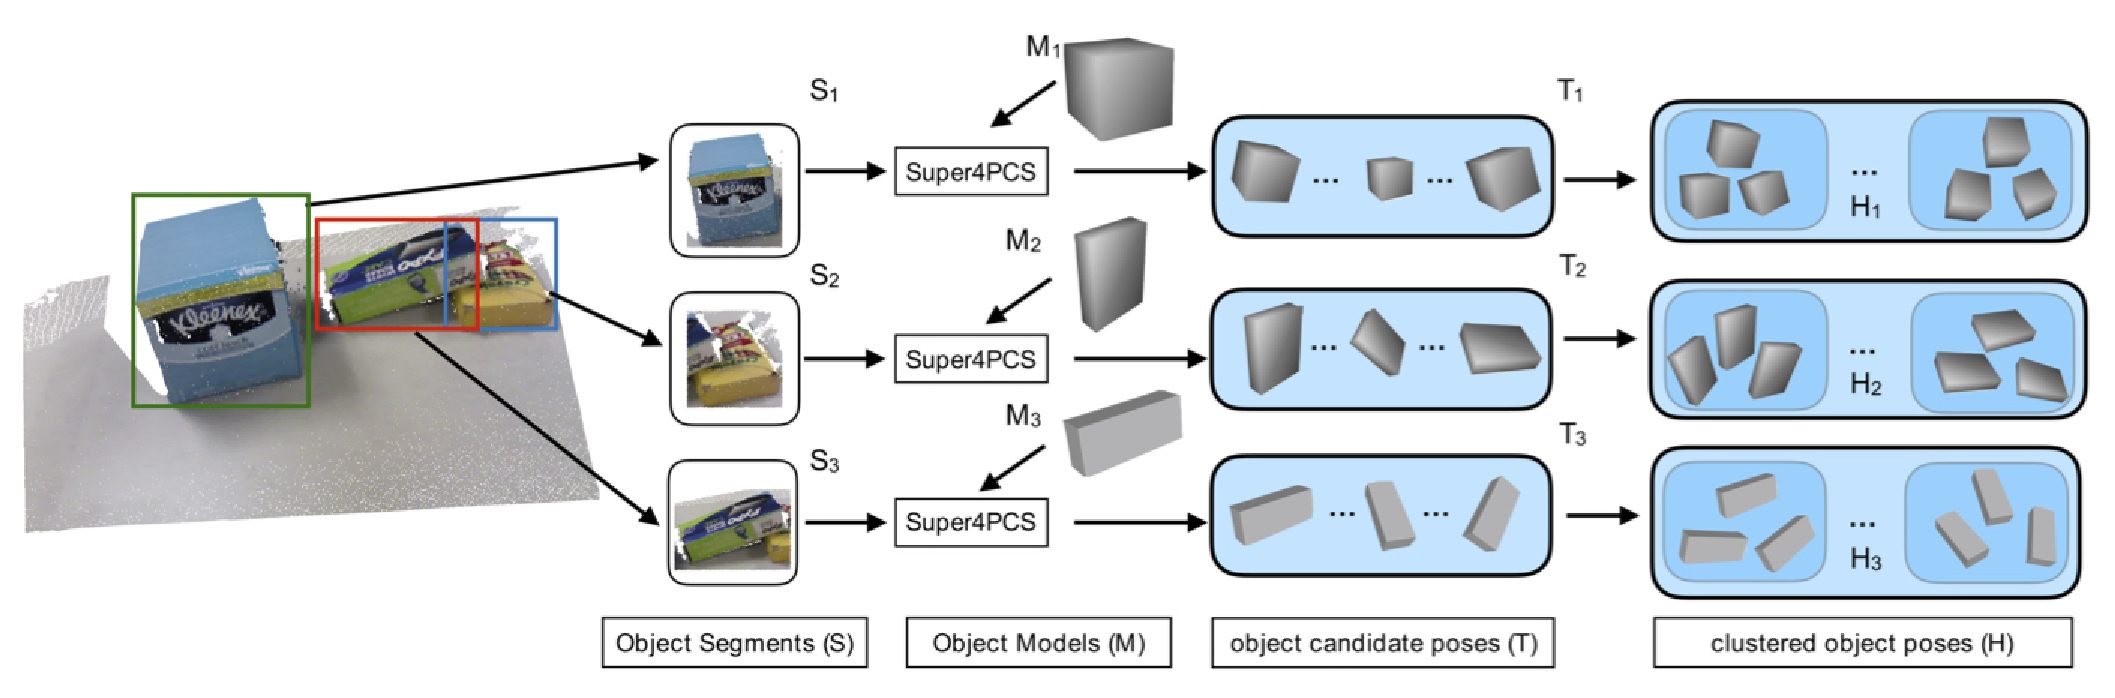
\includegraphics[width=0.9\textwidth]{clustering}
				\caption{object candidate pose generation and clustering to reduce set cardiniality}
			\end{figure}
			\vspace{-0.3in}
			\begin{itemize}
				\item Pose candidate set is constructed for each object using the extracted object segment and the 3D CAD model.
				\item For computational efficiency, the set of object hypotheses is clustered to obtain smaller candidate sets while still containing poses close to the true solutions. 
			\end{itemize}
			\vspace{-0.3in}
			\begin{columns}[t]
			\begin{column} {0.40\textwidth}
			\begin{figure}[h]
				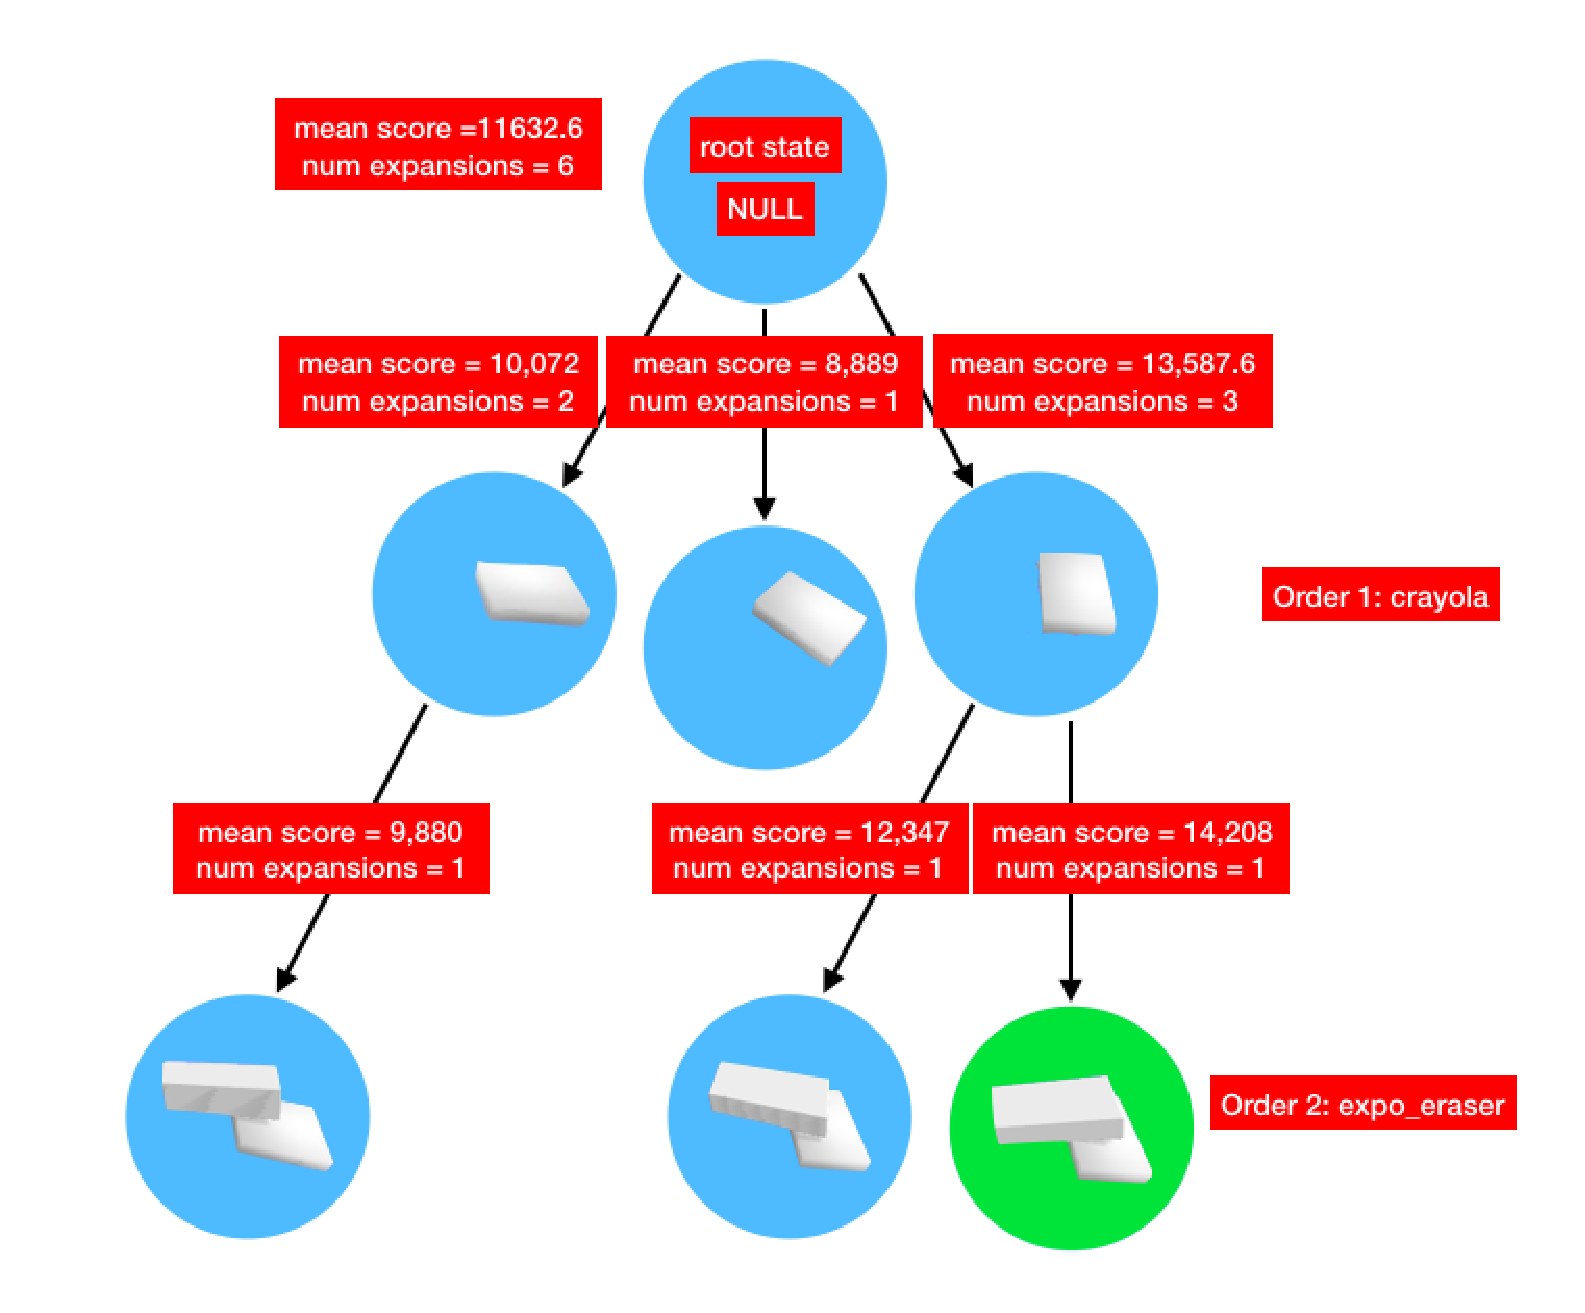
\includegraphics[width=0.8\textwidth]{mcts}
				\caption{Monte Carlo Tree Search for pose estimation}
			\end{figure}
			\end{column}
			\begin{column} {0.60\textwidth}
			\begin{itemize}
				\item An order of object placement is computed based on a set of rules defined over the object segments.
				\item Node expansion in the tree corresponds to an object placement, which is constrained (imposed by using physics simulator and point cloud trimming) by the previously placed objects.
				\item The leaf nodes (complete assignment) are rendered and a score is computed by comparing rendered scene to the observed depth image.
				\item The search uses Upper Confidence Bound to trade-off exploration and exploitation within the search.
			\end{itemize}
			\end{column}
			\end{columns}
		\end{block}
	\end{column}
	\begin{column}{0.30\textwidth}
		\begin{block}{\large Pose Estimation Evaluation}
			\centering
			\begin{itemize}
				\item Results demonstrate that search is useful in case of a clutter.
				\item MCTS converges much faster compared to using a heuristic based on registration score.
			\end{itemize}
			\vspace{-0.2in}
			\begin{figure}[h]
				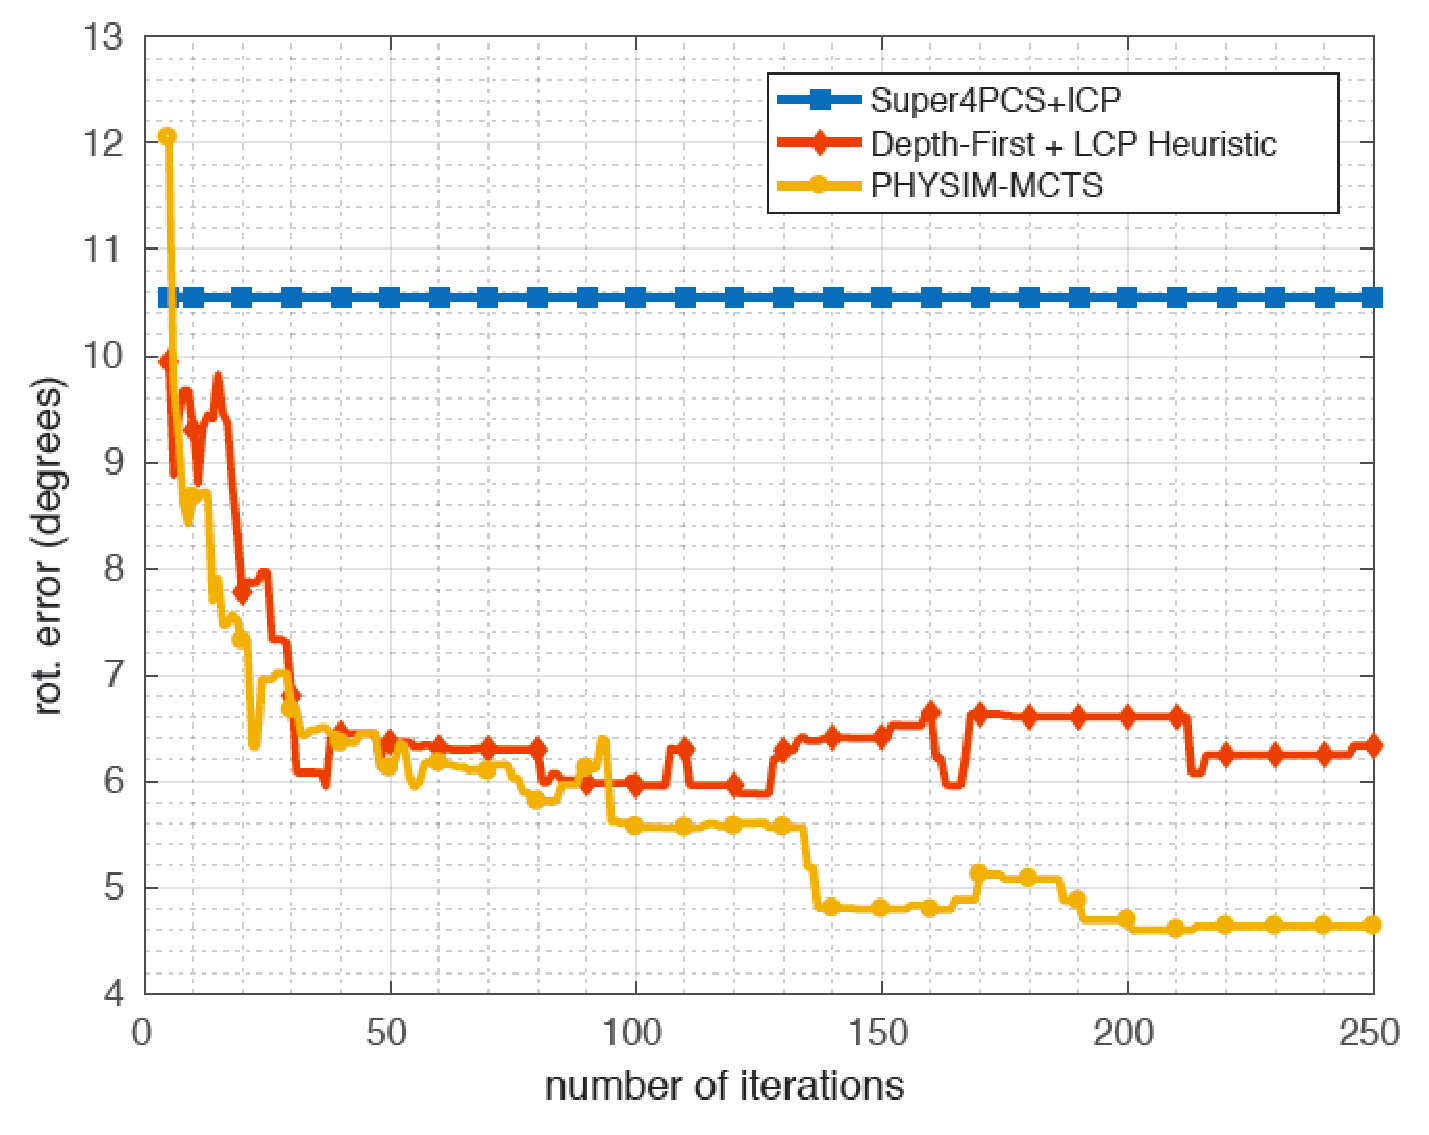
\includegraphics[width=0.75\textwidth]{graph1}
				\caption{Rotation error (degrees) vs the number of search expansions}
			\end{figure}
			\begin{figure}[h]
				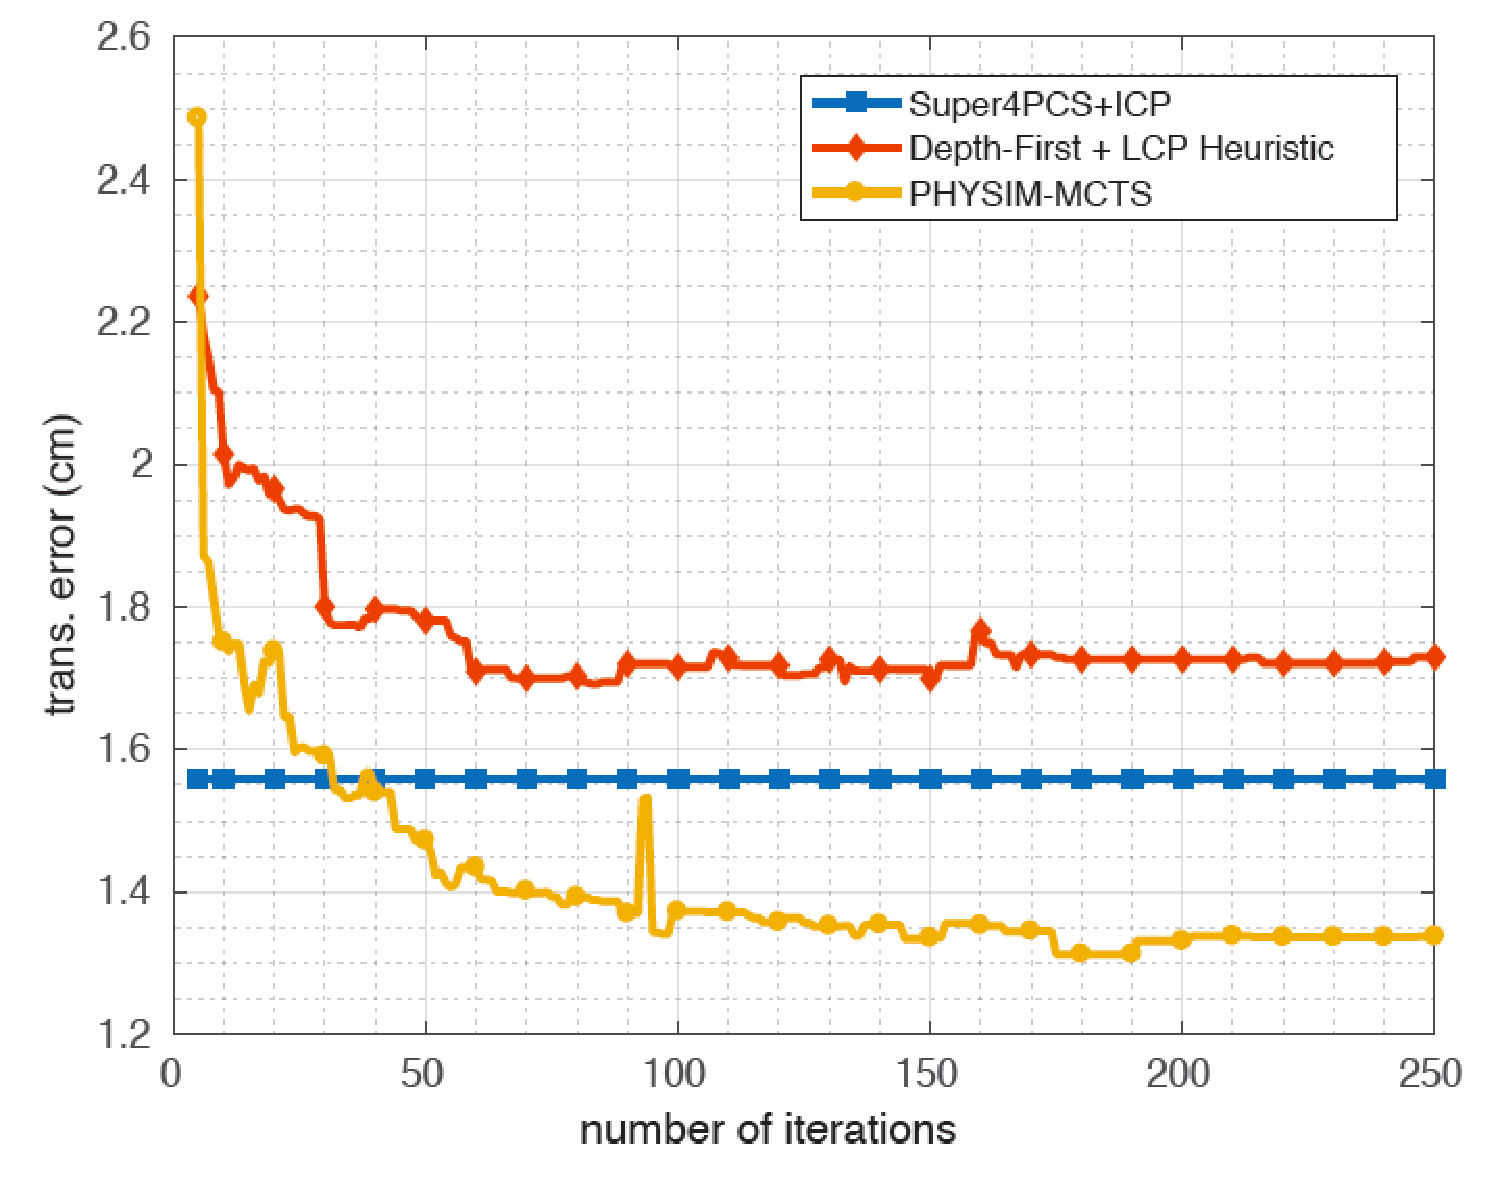
\includegraphics[width=0.75\textwidth]{graph2}
				\caption{Translational error (cms) vs the number of search expansions}
			\end{figure}
		\end{block}
	\end{column}
\end{columns}